\chapter{Vida e Morte}

Nos \emph{Dias. 15 a 18} no \autoref{chap:cinco}, nós brevemente explicamos a diferença entre olhos reais e olhos falsos. Neste capítulo, mostraremos técnicas para a criação de olhos falsos nos grupos adversários, e explicaremos o conceito de olhos falsos.

\section{Olhos Falsos}

\emph{Dia.\@~1.} O grupo preto, que está confinado ao canto, possui somente um olho real, e um olho falso --- o ponto em \textbf{A} ---, portanto ele está morto. No final da partida, se Preto se recusar a aceitar que este grupo está morto, Branco pode demonstrá-lo através dos movimentos no \emph{Dia.\@~2}.

\begin{figure}[h!]
    \centering
    \begin{subfigure}[t]{.31\textwidth}
        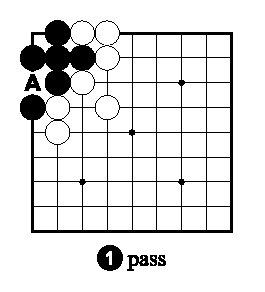
\includegraphics[width=1\textwidth]{8 - False Eyes - Dia 1}
        \caption*{\emph{Dia.\@~1}}
    \end{subfigure}
    \hspace{1cm}
    \begin{subfigure}[t]{.31\textwidth}
        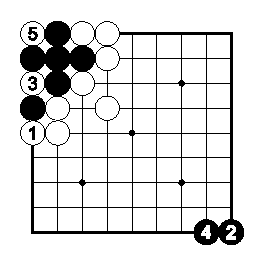
\includegraphics[width=1\textwidth]{8 - False Eyes - Dia 2}
        \caption*{\emph{Dia.\@~2. Preto 2 e 4 passam}}
    \end{subfigure}
\end{figure}

\emph{Dia.\@~2.} Teoricamente, no final da partida, Branco poderá capturar Preto com 1 a 5. Jogadores experientesnão jogariam tais movimentos, eles reconheceriam tal grupo como morto.

\pagebreak

\emph{Dia.\@~3.} Esse grupo preto não está morto ainda, mas Branco pode matá-lo.

\begin{figure}[h!]
    \centering
    \begin{subfigure}[t]{.31\textwidth}
        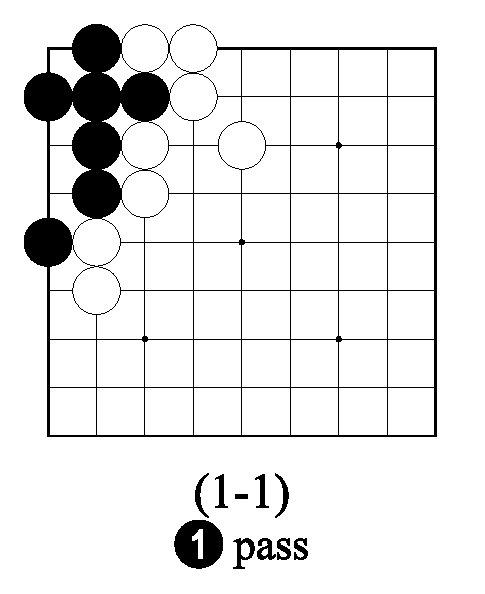
\includegraphics[width=1\textwidth]{8 - False Eyes - Dia 3}
        \caption*{\emph{Dia.\@~3}}
    \end{subfigure}
    \hfill
    \begin{subfigure}[t]{.31\textwidth}
        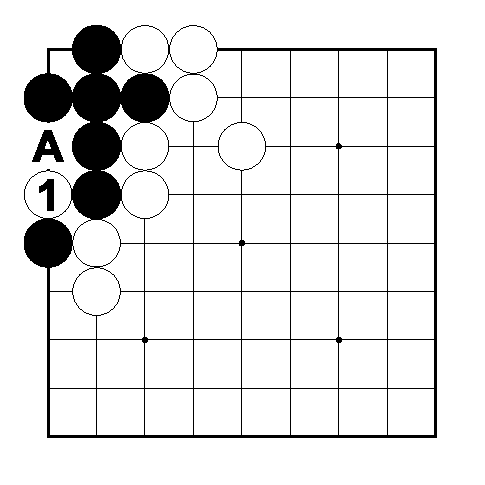
\includegraphics[width=1\textwidth]{8 - False Eyes - Dia 4}
        \caption*{\emph{Dia.\@~4}}
    \end{subfigure}
    \hfill
    \begin{subfigure}[t]{.31\textwidth}
        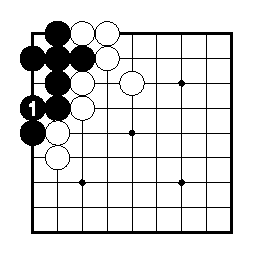
\includegraphics[width=1\textwidth]{8 - False Eyes - Dia 5}
        \caption*{\emph{Dia.\@~5}}
    \end{subfigure}
\end{figure}

\emph{Dia.\@~4.} Branco sacrifica uma pedra com 1, fazendo com que o segundo olho preto se torne falso. Se Preto capturar essa pedra com \textbf{A}, ele acabará com uma posição que é essencialmente idêntica ao \emph{Dia.\@~1}.

\emph{Dia.\@~5.} Para fazer dois olhos, Preto precisa conectar em 1. O grupo preto não poderá, então, mais ser morto.

\pagebreak

\subsection{Exemplo 1}

O grupo preto no \emph{Dia.\@~1} está instável. Ele viverá ou morrerá, dependendo de qual será o próximo movimento.

\begin{figure}[h!]
    \centering
    \begin{subfigure}[t]{.31\textwidth}
        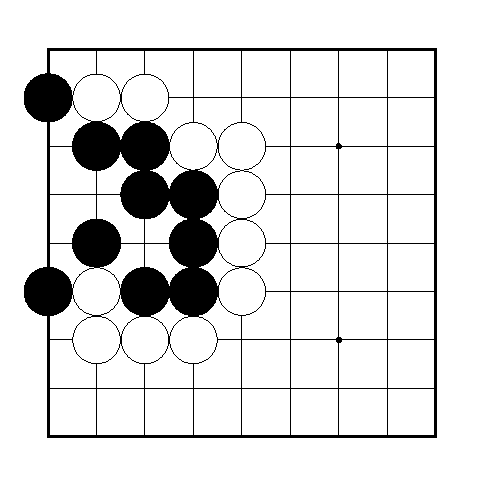
\includegraphics[width=1\textwidth]{8 - False Eyes - Example 1 - Dia 1}
        \caption*{\emph{Dia.\@~1. Instável}}
    \end{subfigure}
    \hspace{1cm}
    \begin{subfigure}[t]{.31\textwidth}
        
\includegraphics[width=1\textwidth]{8 - False Eyes - Example 1 - Dia 2}
        \caption*{\emph{Dia.\@~2. Morto}}
    \end{subfigure}
\end{figure}

Se Branco jogar primeiro, ele matará Preto com a colocação de 1 no \emph{Dia.\@~2}. Se Preto conectar com 2, Branco toma o ponto-chave de 3. Após a captura preta com 4\ldots

Branco sacrifica uma pedra com 5 no \emph{Dia.\@~3}, criando um olho falso naquele ponto. Preto não consegue mais fazer um segundo olho, portanto seu grupo está morto.

\begin{figure}[h!]
    \centering
    \begin{subfigure}[t]{.31\textwidth}
        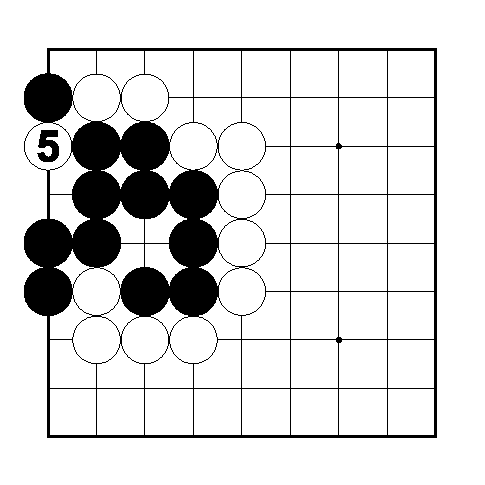
\includegraphics[width=1\textwidth]{8 - False Eyes - Example 1 - Dia 3}
        \caption*{\emph{Dia.\@~3. Morto}}
    \end{subfigure}
    \hspace{1cm}
    \begin{subfigure}[t]{.31\textwidth}
        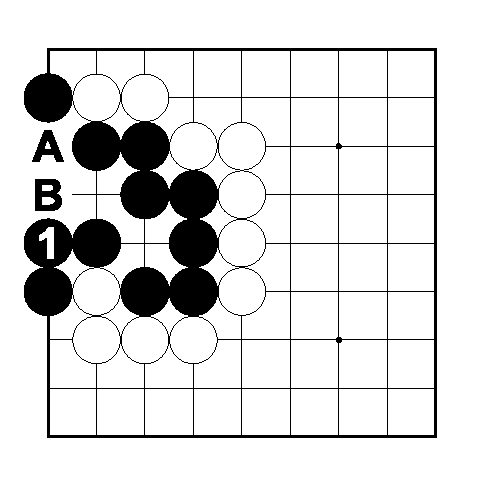
\includegraphics[width=1\textwidth]{8 - False Eyes - Example 1 - Dia 4}
        \caption*{\emph{Dia.\@~4. Vivo}}
    \end{subfigure}
\end{figure}

Se Preto jogar primeiro, ele poderá fazer um segundo olhopara seu grupo pela conexão de 1 no \emph{Dia.\@~4}. Se Branco \textbf{A}, Preto captura em \textbf{B} e obtém seus dois olhos.

\subsection{Exemplo 2}

O grupo preto no \emph{Dia.\@~1} está instável, incompleto. Ele viverá ou morrerá baseado no próximo movimento.

\begin{figure}[h!]
    \centering
    \begin{subfigure}[t]{.31\textwidth}
        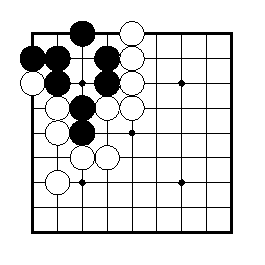
\includegraphics[width=1\textwidth]{8 - False Eyes - Example 2 - Dia 1}
        \caption*{\emph{Dia.\@~1. Instável}}
    \end{subfigure}
    \hspace{1cm}
    \begin{subfigure}[t]{.31\textwidth}
        
\includegraphics[width=1\textwidth]{8 - False Eyes - Example 2 - Dia 2}
        \caption*{\emph{Dia.\@~2. Morto}}
    \end{subfigure}
\end{figure}

Se Branco jogar primeiro, ele poderá matar o grupo preto com o sacrifício de 1 no \emph{Dia.\@~2}. O ponto 1 agora é um olho falso. Capturar com 2 não ajuda Preto a criar um olho. Seu grupo está morto a partir daí.

O ponto \textbf{A} no \emph{Dia.\@~3} é um olho falso. Apesar de que Branco não precisa jogar lá, ele pode forçar Preto a jogar naquele ponto com o atari em \textbf{B}, se desafiado a demonstrar que o grupo Preto está morto.

\begin{figure}[h!]
    \centering
    \begin{subfigure}[t]{.31\textwidth}
        
\includegraphics[width=1\textwidth]{8 - False Eyes - Example 2 - Dia 3}
        \caption*{\emph{Dia.\@~3. Morto}}
    \end{subfigure}
    \hspace{1cm}
    \begin{subfigure}[t]{.31\textwidth}
        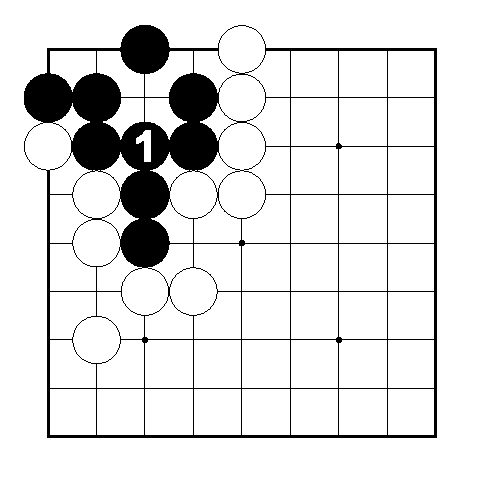
\includegraphics[width=1\textwidth]{8 - False Eyes - Example 2 - Dia 4}
        \caption*{\emph{Dia.\@~4. Vivo}}
    \end{subfigure}
\end{figure}

Se Preto jogar primeiro, ele pode fazer um segundo olho para seu grupo conectando em 1 no \emph{Dia.\@~4}.

\subsection{Exemplo 3}

O grupo preto no \emph{Dia.\@~1} está incompleto. Vida ou morte dependem da próxima jogada.

\begin{figure}[h!]
    \centering
    \begin{subfigure}[t]{.31\textwidth}
        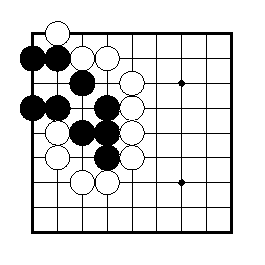
\includegraphics[width=1\textwidth]{8 - False Eyes - Example 3 - Dia 1}
        \caption*{\emph{Dia.\@~1. Instável}}
    \end{subfigure}
    \hspace{1cm}
    \begin{subfigure}[t]{.31\textwidth}
        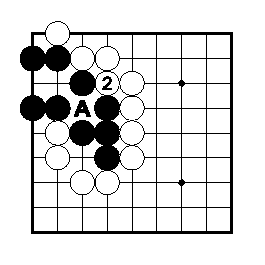
\includegraphics[width=1\textwidth]{8 - False Eyes - Example 3 - Dia 2}
        \caption*{\emph{Dia.\@~2. Morto}}
    \end{subfigure}
\end{figure}

Se Branco jogar primeiro, ele poderá jogar 1 no \emph{Dia 2} e transformar o olho em \textbf{A} em um olho falso. Preto está morto.

\begin{figure}[h!]
    \centering
    \begin{subfigure}[t]{.31\textwidth}
        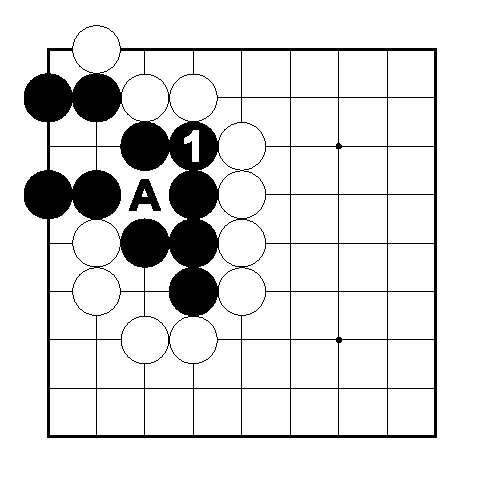
\includegraphics[width=1\textwidth]{8 - False Eyes - Example 3 - Dia 3}
        \caption*{\emph{Dia.\@~1. Vivo}}
    \end{subfigure}
\end{figure}

Se for turno preto, ele pode tornar o ponto \textbf{A} no \emph{Dia.\@~3} em um olho verdadeiro conectando em 1. 

\pagebreak

\section{Espaço de Olho e Forma de Olho}

Quando um grupo cerca um espaço contíguo aberto de vários pontos, a questão de se esse espaço será suficientemente grande para assegurar dois olhos surge.

\emph{Dia.\@~1.} O grupo preto possui um espaço de três intersecções como olho, e seu status é instável.

\begin{figure}[h!]
    \centering
    \begin{subfigure}[t]{.31\textwidth}
        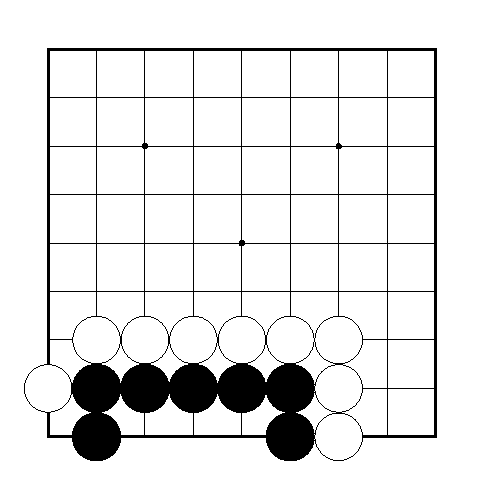
\includegraphics[width=1\textwidth]{8 - Eye Spaces - Dia 1}
        \caption*{\emph{Dia.\@~1}}
    \end{subfigure}
    \hfill
    \begin{subfigure}[t]{.31\textwidth}
        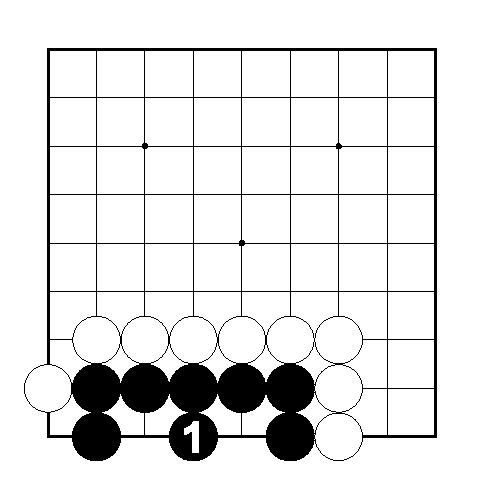
\includegraphics[width=1\textwidth]{8 - Eye Spaces - Dia 2}
        \caption*{\emph{Dia.\@~2}}
    \end{subfigure}
    \hfill
    \begin{subfigure}[t]{.31\textwidth}
        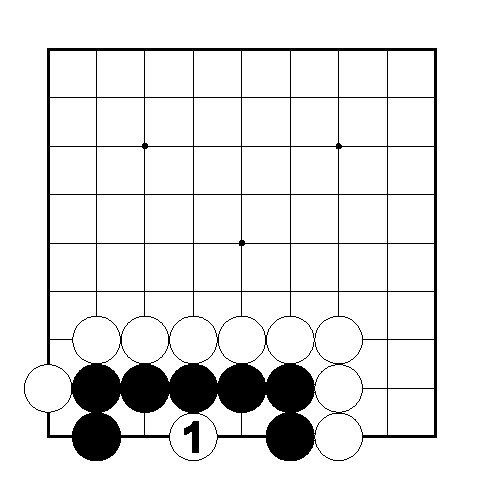
\includegraphics[width=1\textwidth]{8 - Eye Spaces - Dia 3}
        \caption*{\emph{Dia.\@~3}}
    \end{subfigure}
\end{figure}

\emph{Dia.\@~2.} Se Preto jogar 1, ele está vivo, pois possui dois olhos separados.

\emph{Dia.\@~3.} Porém, se Branco jogar 1, Preto está morto.

\begin{figure}[h!]
    \centering
    \begin{subfigure}[t]{.31\textwidth}
        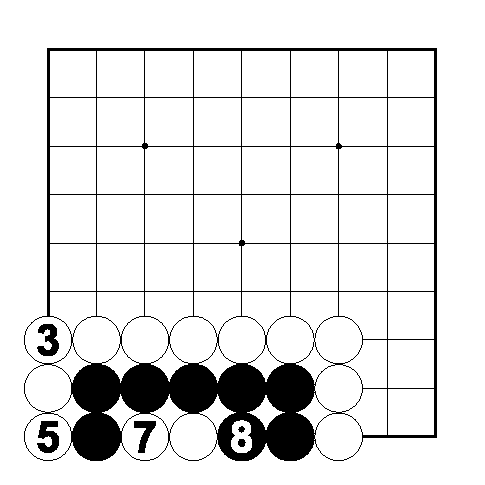
\includegraphics[width=1\textwidth]{8 - Eye Spaces - Dia 4}
        \caption*{\emph{Dia.\@~4}}
    \end{subfigure}
    \hspace{1cm}
    \begin{subfigure}[t]{.31\textwidth}
        
\includegraphics[width=1\textwidth]{8 - Eye Spaces - Dia 5}
        \caption*{\emph{Dia.\@~5}}
    \end{subfigure}
\end{figure}

\emph{Dias. 4 e 5.} Os movimentos até Branco 11 nesses dois diagramas provam que o grupo Preto está morto. Branco simplesmente preenche todas as liberdades pretas mostradas. Preto não tem como se defender.

Aqui seguem mais alguns exemplos.

\emph{Dia.\@~6.} O grupo preto possui um olho de quatro espaços, e está vivo já.

\emph{Dia.\@~7.} Se Branco jogar em 1, Preto joga 2 e, novamente, ele está vivo com dois olhos separados.

\emph{Dia.\@~8.} Similarmente, se Branco jogar 1, Preto jogará 2 e, novamente, ele estará vivo com dois olhos separados.

\begin{figure}[h!]
    \centering
    \begin{subfigure}[t]{.31\textwidth}
        
\includegraphics[width=1\textwidth]{8 - Eye Spaces - Dia 6}
        \caption*{\emph{Dia.\@~6}}
    \end{subfigure}
    \hfill
    \begin{subfigure}[t]{.31\textwidth}
        
\includegraphics[width=1\textwidth]{8 - Eye Spaces - Dia 7}
        \caption*{\emph{Dia.\@~7}}
    \end{subfigure}
    \hfill
    \begin{subfigure}[t]{.31\textwidth}
        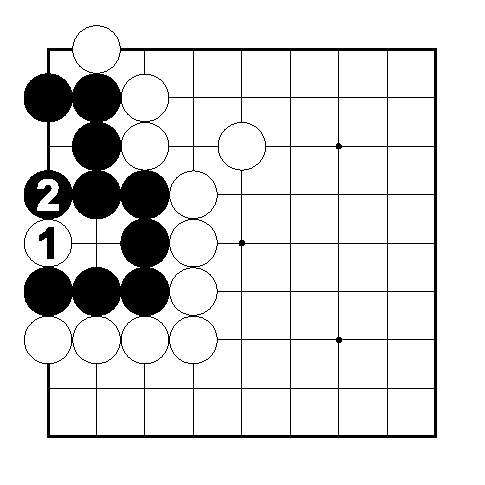
\includegraphics[width=1\textwidth]{8 - Eye Spaces - Dia 8}
        \caption*{\emph{Dia.\@~8}}
    \end{subfigure}
\end{figure}

\pagebreak

\emph{Dia.\@~9.} Após Branco 1, Preto não pode passar ou ignorar o movimento branco. Branco continuará com 3 e Preto morrerá.

\begin{figure}[h!]
    \centering
    \begin{subfigure}[t]{.31\textwidth}
        
\includegraphics[width=1\textwidth]{8 - Eye Spaces - Dia 9}
        \caption*{\emph{Dia.\@~9. Preto 2 passa}}
    \end{subfigure}
    \hfill
    \begin{subfigure}[t]{.31\textwidth}
        
\includegraphics[width=1\textwidth]{8 - Eye Spaces - Dia 10}
        \caption*{\emph{Dia.\@~10. Preto 4, 6 e 8 passam}}
    \end{subfigure}
    \hfill
    \begin{subfigure}[t]{.31\textwidth}
        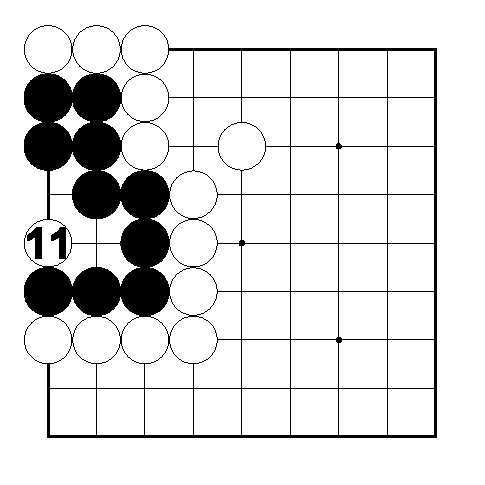
\includegraphics[width=1\textwidth]{8 - Eye Spaces - Dia 11}
        \caption*{\emph{Dia.\@~11}}
    \end{subfigure}
\end{figure}

\emph{Dia.\@~10.} Branco pode demonstrar que Preto está morto jogando 5 a 9. Depois da captura por Preto em 10\ldots

\emph{Dia.\@~11.} Branco joga em 11, e a situação se torna clara: Preto não possui dois olhos.

\begin{figure}[h!]
    \centering
    \begin{subfigure}[t]{.31\textwidth}
        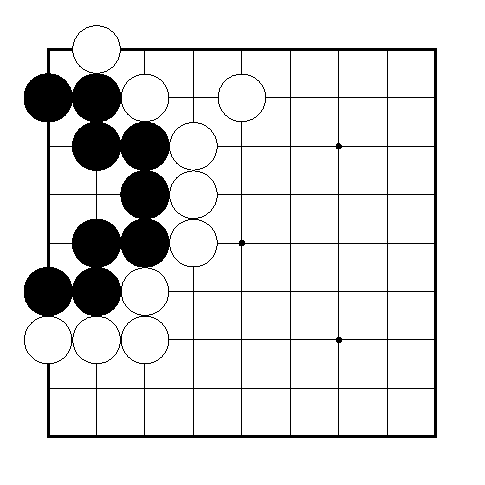
\includegraphics[width=1\textwidth]{8 - Eye Spaces - Dia 12}
        \caption*{\emph{Dia.\@~12}}
    \end{subfigure}
    \hfill
    \begin{subfigure}[t]{.31\textwidth}
        
\includegraphics[width=1\textwidth]{8 - Eye Spaces - Dia 13}
        \caption*{\emph{Dia.\@~13}}
    \end{subfigure}
    \hfill
    \begin{subfigure}[t]{.31\textwidth}
        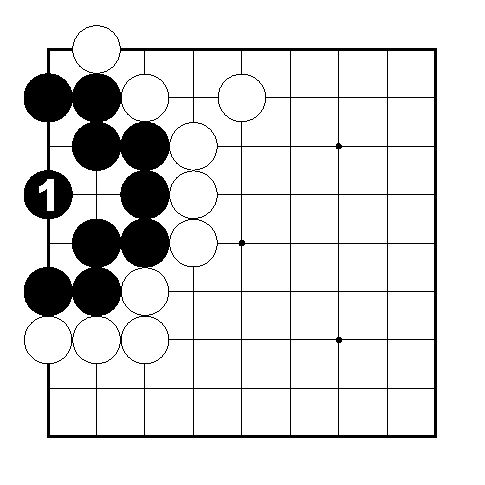
\includegraphics[width=1\textwidth]{8 - Eye Spaces - Dia 14}
        \caption*{\emph{Dia.\@~14}}
    \end{subfigure}
\end{figure}

\emph{Dia.\@~12.} O grupo preto está vivo ou morto, dependendo de quem for a vez.

\emph{Dia.\@~13.} Se for turno branco, e ele jogar em 1, o grupo preto está morto.

\emph{Dia.\@~14.} Se for turno preto, ele pode fazer três olhos jogando em 1.

\pagebreak

\emph{Dia.\@~15.} O grupo preto é um quadrado de quatro espaços, e está morto já.

\emph{Dia.\@~16.} Mesmo se Preto jogar primeiro, tudo que ele pode fazer é jogar em 1 (ou qualquer outro ponto simétrico) e ameaçar fazer dois olhos jogando em 2. No entanto, Branco pode jogar 2 primeiro, e Preto é deixado sem uma resposta. Se ele jogar qualquer um entre \textbf{A} ou \textbf{B}, ele coloca todo seu grupo em atari.

\begin{figure}[h!]
    \centering
    \begin{subfigure}[t]{.31\textwidth}
        
\includegraphics[width=1\textwidth]{8 - Eye Spaces - Dia 15}
        \caption*{\emph{Dia.\@~15}}
    \end{subfigure}
    \hfill
    \begin{subfigure}[t]{.31\textwidth}
        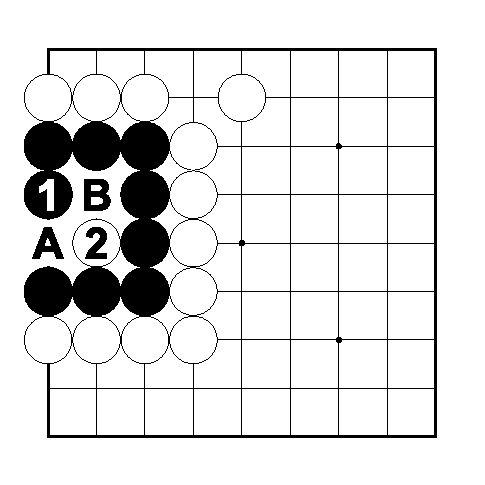
\includegraphics[width=1\textwidth]{8 - Eye Spaces - Dia 16}
        \caption*{\emph{Dia.\@~16}}
    \end{subfigure}
    \hfill
    \begin{subfigure}[t]{.31\textwidth}
        
\includegraphics[width=1\textwidth]{8 - Eye Spaces - Dia 17}
        \caption*{\emph{Dia.\@~17}}
    \end{subfigure}
\end{figure}

\emph{Dia.\@~17.} Se Branco for desafiado a provar que o grupo Preto está morto, tudo que ele precisa fazer é jogar o atari em 4. Se Preto 5 capturar, Branco 6 joga novamente em 4, e todo o grupo preto inevitavelmente será capturado.

\emph{Dia.\@~18.} O grupo preto está vivo ou morto, dependendo de quem for o turno.

\begin{figure}[h!]
    \centering
    \begin{subfigure}[t]{.31\textwidth}
        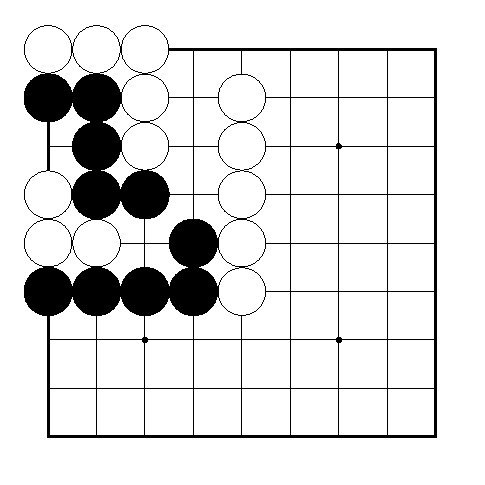
\includegraphics[width=1\textwidth]{8 - Eye Spaces - Dia 18}
        \caption*{\emph{Dia.\@~18}}
    \end{subfigure}
    \hfill
    \begin{subfigure}[t]{.31\textwidth}
        
\includegraphics[width=1\textwidth]{8 - Eye Spaces - Dia 19}
        \caption*{\emph{Dia.\@~19}}
    \end{subfigure}
    \hfill
    \begin{subfigure}[t]{.31\textwidth}
        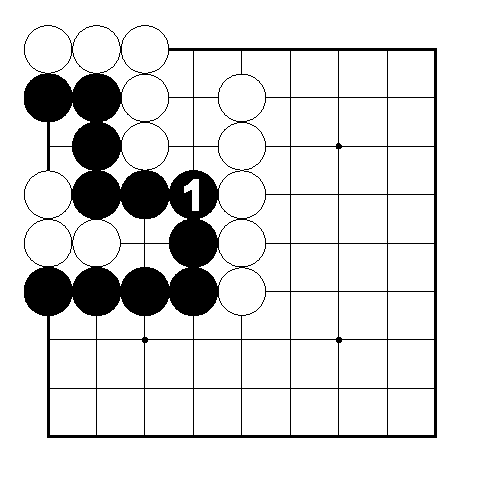
\includegraphics[width=1\textwidth]{8 - Eye Spaces - Dia 20}
        \caption*{\emph{Dia.\@~20}}
    \end{subfigure}
\end{figure}

\emph{Dia.\@~19.} Se Branco jogar primeiro, ele pode matar Preto com 1. Esse movimento põe as cinco pedras pretas em atari. Se Preto conectar em \textbf{A}, todas as pedras estarão em atari. Após Branco 1, o grupo preto está morto, e a posição já está sedimentada.

\emph{Dia.\@~20.} Se for turno preto, ele pode viver jogando no ponto-chave de 1. Preto está vivo em seki. A posição fica como está. No final da partida, as três pedras brancas permanecerão no tabuleiro, e tanto Preto quanto Branco receberão zero pontos de território nesta região.

\pagebreak

\begin{figure}[h!]
    \centering
    \begin{subfigure}[t]{.31\textwidth}
        
\includegraphics[width=1\textwidth]{8 - Eye Spaces - Dia 21}
        \caption*{\emph{Dia.\@~21}}
    \end{subfigure}
    \hspace{1cm}
    \begin{subfigure}[t]{.31\textwidth}
        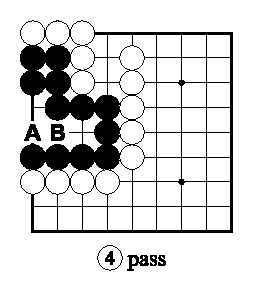
\includegraphics[width=1\textwidth]{8 - Eye Spaces - Dia 22}
        \caption*{\emph{Dia.\@~22}}
    \end{subfigure}
\end{figure}

\emph{Dia.\@~21.} Se Branco resistir respondendo Preto 1, no \emph{Dia.\@~20}, com 2, Preto captura as quatro pedras brancas com 3.

\emph{Dia.\@~22.} Esse é o resultado da captura das pedras brancas no \emph{Dia.\@~21}. Preto está vivo com quatro pontos de território mais quatro pedras capturadas. Se Branco \textbf{A}, Preto ganha dois olhos jogando em \textbf{B}. Se Branco \textbf{B}, Preto \textbf{A}. Resistir, como no \emph{Dia.\@~21}, é uma perda de oito pontos para Branco.

\emph{Dia.\@~23.} O grupo preto possui um olho de cinco espaços. Ele está vivo ou morto, dependendo de quem for o turno.

\begin{figure}[h!]
    \centering
    \begin{subfigure}[t]{.31\textwidth}
        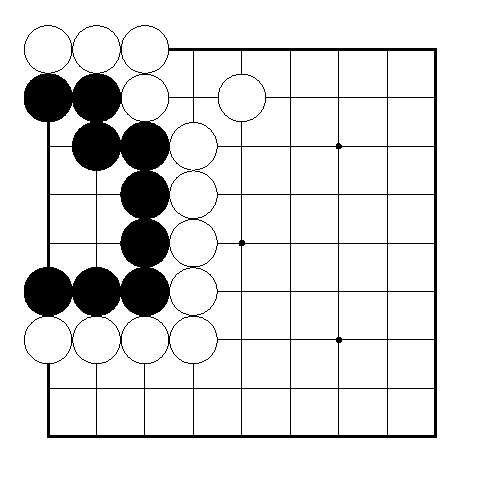
\includegraphics[width=1\textwidth]{8 - Eye Spaces - Dia 23}
        \caption*{\emph{Dia.\@~23}}
    \end{subfigure}
    \hfill
    \begin{subfigure}[t]{.31\textwidth}
        
\includegraphics[width=1\textwidth]{8 - Eye Spaces - Dia 24}
        \caption*{\emph{Dia.\@~24}}
    \end{subfigure}
    \hfill
    \begin{subfigure}[t]{.31\textwidth}
        
\includegraphics[width=1\textwidth]{8 - Eye Spaces - Dia 25}
        \caption*{\emph{Dia.\@~25}}
    \end{subfigure}
\end{figure}

\emph{dia. 24.} Depois de Branco 1, não mais nenhuma maneira com que Preto possa fazer dois olhos. Se necessário realmente capturar o grupo, Branco pode colocá-lo sob atari ocupando as intersecções marcadas com \textbf{X}. Se Preto, então, capturar com \textbf{A}, Preto acaba com um olho de quatro espaços, que é a mesma posição do \emph{Dia.\@~15}, onde mostramos que o grupo Preto está morto já.

\emph{Dia.\@~25.} Se for turno preto, ele poderá fazer dois olhos jogando no ponto-chave de 1.

O tópico de espaço de olho é minuciosamente contemplado no livro \emph{The Basics of Life and Death}~\cite{zeijst_bozulich_basics_of_life_and_death}, publicado pela Kiseido.